\chapter{Blockchain}

\textbf{NB: devi parlare anche della puzzle frendliness (compatibilità con i puzzle)}

Le cryptomonete, a partire dal 2018\foot{Anno di pubblicazione del whitepaper di Satoshi Nakamoto}, hanno ricevuto molte attenzioni da coloro che sono interessati ad investirici o costruire nuovi servizi per un guadagno personale ma soprattutto è esploso l'interesse verso la vera innovazione tecnologica su cui sono basate tutte le criptomonete: la \textbf{blockchain}.

Una \textit{blockchain} può essere pensata come un database distribuito che è replicato in diversi computer connessi ad una rete.\newline
La principale innovazione introdotta da questa tecnologia è nel protocollo usato per gestire transazioni anche su reti a bassa latenza o dispositivi a bassa potenza senza la necessità di un sistema centrale per garantire protezione e affidabilità.

Non esiste una definizione globalmente valida di \textit{Blockchain} a causa delle differenti implementazioni e varianti ma è possibile delineare alcuni punti chiave.
Una blockchain è una rete \textit{peer-to-peer} completamente \textit{distribuita} che fa ampio uso di crittografia per eseguire applicazioni, salvare dati, trasferire asset digitali in maniera \textit{sicura}; questa tecnologia può essere vista come un registro, pubblico e non controllato da nessuna autorità centrale in cui è solo possibile aggiungere dati (\textbf{append-only}).

Questa definizione è interessante in quanto non menziona nessun termine finanziaro o particolari casi d'uso e non specifica protocolli o algoritmi di consenso in quanto una blockchain può essere implementata come un sistema general purpose e non come solo meccanismo per i pagamenti elettronici; infatti, la prima blockchain è stata progettata nel 1991 da due crittografi: \texit{Stuart Haber} e \textit{Scott Stornetta} per firmare dei documenti digitali per prevenire modifiche illecite dei dati e autenticazione.

\section{Storia}

La blockchain utilizzata per i Bitcoin è la prima modera blockchain ad essere utilizzata per pagamenti elettronici sicuri, distribuiti ed anonimi ed è stata presentata da Satoshi Nakamoto nel 2008. L'esigenza di Satoshi era quella di creare un protocollo decentralizzato per coniare una moneta digitale senza il bisogno di una figura centrale di fiducia ed evitare il problema del double-spending di possibili attori malevoli.
Molte altre proposte sono state fatte prima dei Bitcoin ma nessuna risolveva a pieno i problemi di decentralizzazione e consenso distribuito.

La prima blockchain conosciuta, però, non è quella implementata per Bitcoin e non è stata usata per pagamenti elettronici ma come metodo di validazione per documenti digitali nel 1991.

\subsection{Haber e Stornetta}

L'idea di Haber e Stornetta\cite{haberstornetta} era di certificare la data di creazione o modifica di un documento; per esempio, in materia di dispute pre la proprietà intelletuale è cruciale verificare la data di un prototipo brevettabile: la soluzione richiedere di risolvere due problemi:
\begin{itemize}
    \item la data e l'ora dovrebbero far parte del timestamp e non solo nel documento;
    \item prevenire ogni modifica del timestamp e quindi del documento.
\end{itemize}
La soluzione proposta dai due crittografi permette di eseguire un timestamp digitale dei documenti in modo tale che sia infattibile pe un attaccante alterare questi dati.\newline
Il processo di timestamp di un documento prevede l'utilizzo di funzioni di hashing crittografiche: $h: \{0,1\}^* -> \{0,1\}^l$.\newline
A differenza delle funzioni di hashing presentate nel capitolo \ref{sec:funzioni-hashing} non è necessario che siano resistenti alla seconda preimmagine in quanto la soluzione richiede che da un hash non sia possibile risalire al messaggio originale.
Utilizzando le funzioni di hashing è possibile quindi evitare di fornire l'intero documento ad un servizio per timestamp e quindi garantire la privacy del documento stesso: il contenuto intelletuale non è divulgato pubblicamente.\newline
Una volta che l'hash del documento è stato generato è possibile applicargli una firma digitale.\newline

Una prima soluzione proposta prevede l'utilizzo di servizio di terze parti (\textit{Time-Stamping Service}) per elaborare e firmare il documento ma sorge il problema della falsificazione: è necessario implementare una soluzione che sia assente da terze parti per garantire il massimo della fiducia.
\begin{figure}
    \centering
    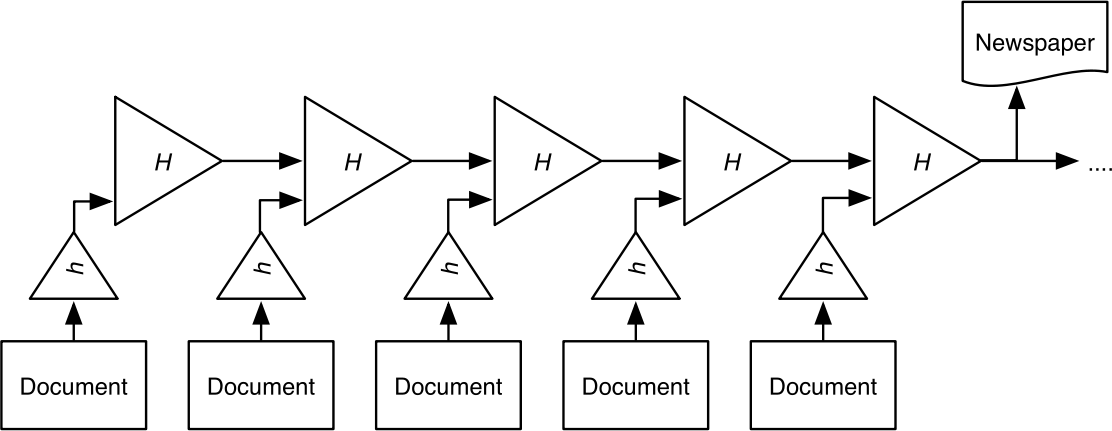
\includegraphics[width=\textwidth]{images/haberstornetta.png}
    \caption{Linking di documenti presso un servizio di timestamp}
    \label{fig:haberstornetta}
\end{figure}
Due possibili scenario possono essere realizzati o combinati:
\begin{enumerate}[1.]
    \item utilizzare un servizio di timestamp (\textit{TTS}) non fidato ma che sia obbligato a produrre timestamp genuini utilizzando il \textit{linking};
    \item distribuire la computazione tra diversi utenti del servizio (\textit{decentralizzazione}).
\end{itemize}
Tramite \textit{linking} gli hash dei documenti presentati al servizio sono collegati come in figura \ref{fig:haberstornetta} e il risultato finale è reso pubblico agli utenti. La seconda soluzione prevede che alcuni utenti, scelti randomicamente, producano il timestamp dell'hash.

Una implementazione della blockchain di Haber e Stornetta è attiva dal 1995: l'azienda \textit{Surety}\footnote{\href{http://surety.com}{Surety}} ogni settimana pubblica una stringa in \textit{base 16} dell'hash di tutte le nuove signature dei clienti della settimana sulla rivista \textit{New York Times}.
\begin{figure}[H]
    \centering
    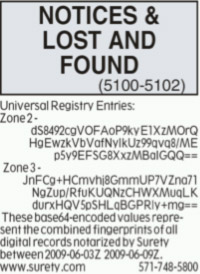
\includegraphics[width=0.35\textwidth]{images/nyt.jpg}
    \caption{Esempio del \textit{base 16} pubblicato sul New York Time da Surety}
    \source{Surety}
\end{figure}

\subsection{Blockchain come sistema di pagamento}
L'implementazione teorica della blockchain di Haber e Stornetta è molto simile a quella presentata nel whitepaper di Satoshi Nakamoto\cite{bitcoin}, infatti, tre degli otto paper citati nel documento \textit{Bitcoin: A Peer-to-Peer Electronic Cash System} sono scritti proprio da Haber e Stornetta\footnote{In quanto l'identità di Satoshi non è mai stata svelata questo fatto ha alimentato voci per cui proprio i due crittografi siano i creatori dei Bitcoin, vedi appendice \ref{app:satoshi}.}.\newline
L'obiettivo di Satoshi era quello di creare un sistema di pagamento elettronico decentralizzato con un forte utilizzo della crittografia, lo stesso che ha portato alla creazione, tra gli anni '90 e 2000, di \textit{eCash}, \textit{SET}, \textit{Hashcash} e \textit{b-cash}. Tutte queste proposte hanno riscontrato dei problemi per cui non era sicuro utilizzarle ma che hanno dato spunto e suggerimenti a Nakamoto.

\section{Struttura}
Una blockchain è un lista di record, chiamati blocchi, che sono collegati tramite l'utilizzo di tecniche crittografiche e che permette solo azioni di inserimento. Ogni record o blocco contiene la informazioni sulle transazioni effettuate tra gli utenti.
In questo modo la lista dei blocchi rappresenta uno storico (registro) di tutte le transazioni che sono state fatte e quindi è anche possibile risalire al bilancio totale di ciascun utente.
In quanto non esiste una definizione ed implementazione globalmente valida di blockchain verrà presentata quella utilizzata per i Bitcoin come generica.

Una blockchain è generalmente composta da alcuni elementi fondamentali:
\begin{itemize}
    \item blocco;
    \item nodo;
    \item transazione.
\end{itemize}

\subsection{Blocco}
Un blocco è un singolo elemento della lista formata da tutti i record componenti la blockchain.
\begin{figure}[H]
    \centering
    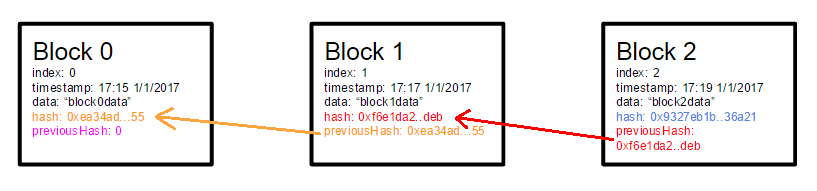
\includegraphics[width=\textwidth]{images/blockchain_basic.png}
    \caption{Esempio di blockchain formata da tre blocchi}
\end{figure}
I blocchi sono connessi come una lista tramite l'utilizzo delle funzioni di hashing e quindi, per design, sono resistenti alla modifica dei dati.
Ogni blocco contiene come dato l'hash del blocco che lo precede nella lista, un timestamp, un indice e i dati che devono essere memorizzati permanentemente.\newline
La crittografia fornisce sia autenticazione che verifica ed è usata per garantire un sistema di computazione sicuro senza un singolo proprietario o sistema centrale.\newline
Il primo nodo della lista è chiamato \textit{genesi} in quanto partendo da quello verrà creata la lista che compone la blockchain. Nella maggior parte delle implementazioni questo blocco è inserito nel codice sorgente, non produce o consuma dati e non è collegato a nessun precedente blocco.

Blocks are linked using cryptography and by design are resistant to data modification. Cryptography provides authentication and verification and is used to conjure a secure computing environment out of many nodes without central authority or single owner.\\
Each block contains a cryptographic hash of the previous block, a timestamp and the data to store in a permanent way.

Each block contains a cryptographic hash of the previous block,[6] a timestamp, and transaction data (generally represented as a merkle tree root hash). By design, a blockchain is resistant to modification of the data. It is "an open, distributed ledger that can record transactions between two parties efficiently and in a verifiable and permanent way".[8] For use as a distributed ledger, a blockchain is typically managed by a peer-to-peer network collectively adhering to a protocol for inter-node communication and validating new blocks. Once recorded, the data in any given block cannot be altered retroactively without alteration of all subsequent blocks, which requires consensus of the network majority.

Though blockchain records are not unalterable, blockchains may be considered secure by design and exemplify a distributed computing system with high Byzantine fault tolerance. Decentralized consensus has therefore been claimed with a blockchain.[9]

Blockchain was invented by Satoshi Nakamoto in 2008 to serve as the public transaction ledger of the cryptocurrency bitcoin.[1] The invention of the blockchain for bitcoin made it the first digital currency to solve the double-spending problem without the need of a trusted authority or central server. The bitcoin design has inspired other applications.[1][3]


% NeoTex: mainfile=main.tex:
